\documentclass[notitlepage]{report}
\usepackage[left=0.5in, right=0.5in, top=0.5in, bottom=0.5in]{geometry}
\usepackage[parfill]{parskip}

\usepackage{graphicx}
\graphicspath{ {C:/Users/PaulB/Documents/msba/CIS_508/images/assignment_one/} }

\usepackage{titling}
\usepackage{lipsum}
\usepackage{float}
\usepackage{setspace}

\pretitle{\begin{center}\Huge\bfseries}
\posttitle{\par\end{center}\vskip 0.5em}
\preauthor{\begin{center}\Large\ttfamily}
\postauthor{\end{center}}
\predate{\par\large\centering}
\postdate{\par}
\doublespacing

\pagenumbering{gobble}

\title{CIS 508 Individual Assignment \#1}
\author{Paul Bernert}
\date{September 6, 2020}
\begin{document}

\maketitle
\thispagestyle{empty}

\section*{Santander Customer Satisfaction}
A recently concluded Kaggle competition had a prize of \$60,000 and was about predicting customer satisfaction. Download the training and test sets from the Kaggle site and train and validate a decision tree classification model from the Scikit-learn machine learning library. The training and test sets are also provided.

You can change the default parameters of the decision tree classifier to explore other solutions. Explore at least three other solutions by changing the parameters of the decision tree classifier, such as depth of tree, splitting criterion and maximum number of leaf nodes. Use screenshots of Python code to explain what parameters you changed and why.

In your report, discuss some of the major characteristics of the dataset / problem using the ideas of Exploratory Data Analysis. Also explain why this is a hard problem from a machine learning point of view. 

Do Kaggle submissions of your test results from different decision tree models and record all Kaggle scores / rankings in your report.

\section*{Solution}
The objective of this homework assignment is to take a training dataset, construct several different Decision Tree models and determine whether we are able to have relative success in predicting target values in a testing dataset. Our results will be submitted to Kaggle, where the accuracy of our work will be presented.

We first start with the training dataset, which is split into training and testing sub-datasets (in the models below, a 75\%-to-25\% training-to-testing split was used). With the training sub-dataset, we can construct a series of Decision Tree models to determine which parameters ask "the best set of questions". Once we have created a model, we test our accuracy of the model against the test sub-dataset. If the model seems reasonable (high enough accuracy or low GINI scores without being overfit), we can then use the model against the full test dataset. Those results are sent to Kaggle for scoring.

A model is created using \textit{sklearn}, a library within Python that contains several different machine learning functions. The one we are using on this assignment is the \textit{DecisionTreeClassifier} function.

Once a model is created, you then must fit data. Since we have already split the data (within the training dataset), we can simply fit the data by doing \textit{x.fit(X\_train,y\_train)}, where x is the name of your model.

Finally, we can use the model with the fit data to predict values. Once you've done this and things seem to make sense, we can cast that to the testing dataset to get a final output.

\subsection*{Model One}
The first model tested uses the default parameters for the DecisionTreeClassifer function:

$$
DecisionTreeClassifier()
$$

A decision tree model using no parameters and the provided data can be visualized as:

\begin{figure}[H]
	\centering
	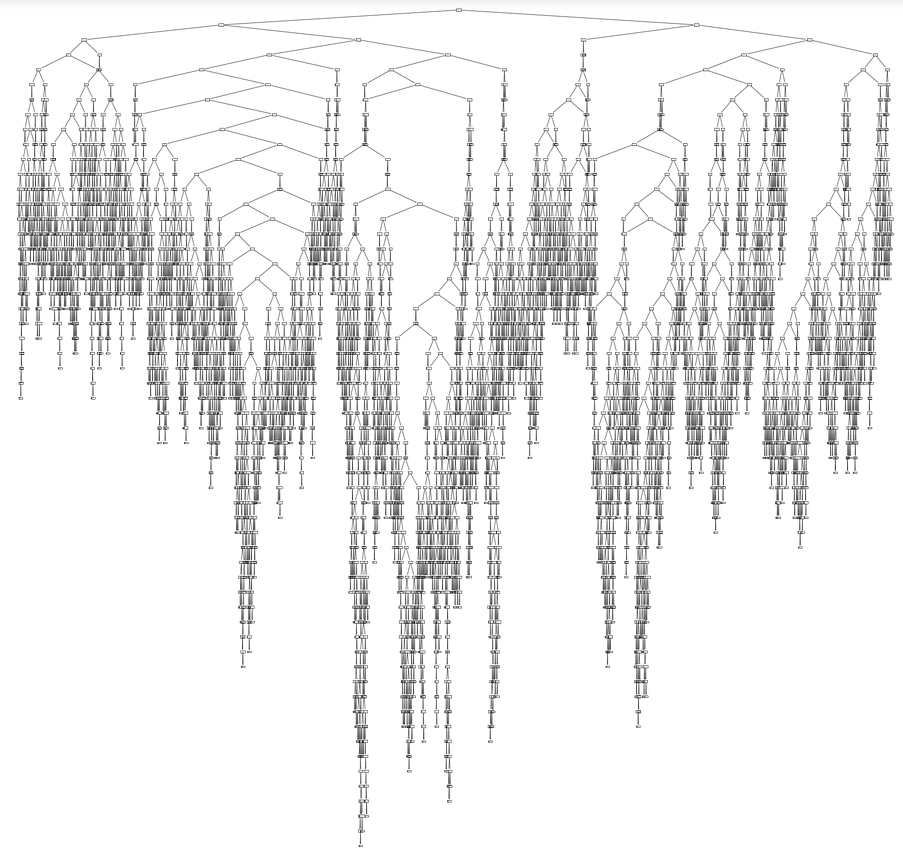
\includegraphics[width=6.5in]{model_1.png}
\end{figure}

This model has a 93.2\% accuracy when predicting target values of the testing sub-dataset. This model is generally considered an overfit model, because it has essentially created a glorified lookup table. The leaf nodes will never contain more than 2 samples, and will usually have one sample [0,1]. If you work down the tree and ask every question until you reach the bottom, you will usually only have 1 row in the dataset that matches those critera. This is objectively a bad model, because while it may be able to predict itself (the training sub-set), the questions it has assigned will generally not be able to accurately predict new data.

\subsection*{Model Two}
The second model uses the following parameters in the DecisionTreeClassifier function:

$$
DecisionTreeClassifier(min\_samples\_split=1000)
$$

A decision tree model using the parameters established in Model 2 can be visualized as so:

\begin{figure}[H]
	\centering
	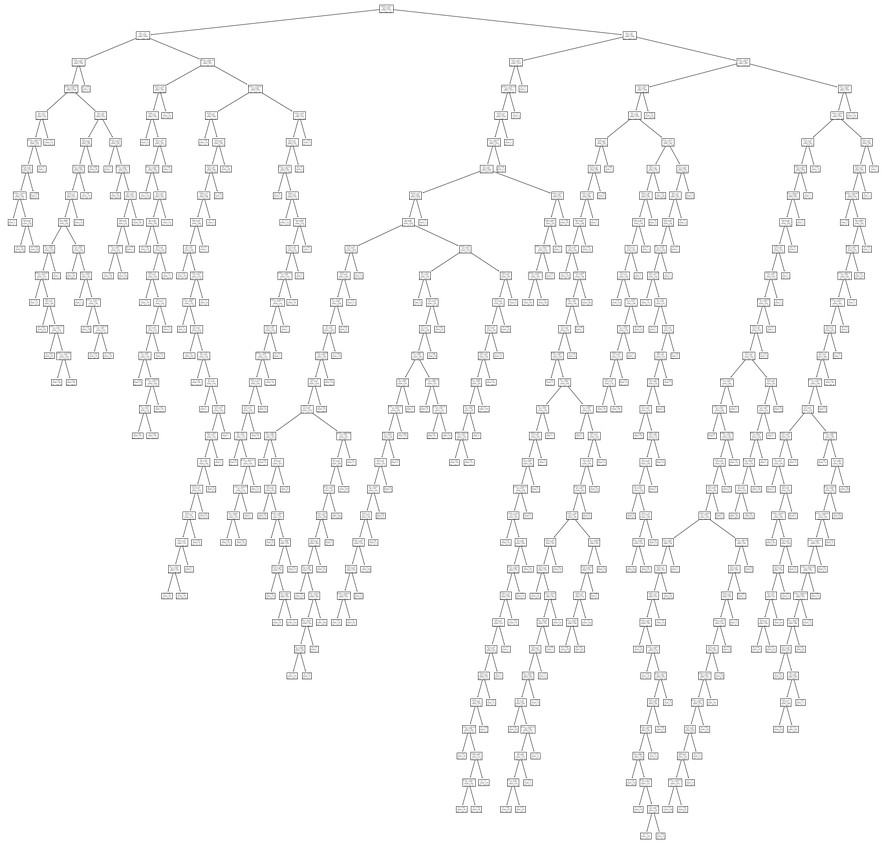
\includegraphics[width=6.5in]{model_2.png}
\end{figure}

We added one parameter in this model: \textit{min\_sample\_split=1000}. This essentially means that once a node has less than (or equal to) 1,000 samples, it will not continue to ask additional questions and create new nodes. This is one of the simplest ways to combat overfitting the data. This model has an accuracy of 96.0\%.

\subsection*{Model Three}
The third model tested uses the following parameters in the DecisionTreeClassifier function:

$$
DecisionTreeClassifier(min\_samples\_split=5702)
$$

A decision tree model using the parameters established in Model 3 can be visualized as so:

\begin{figure}[H]
	\centering
	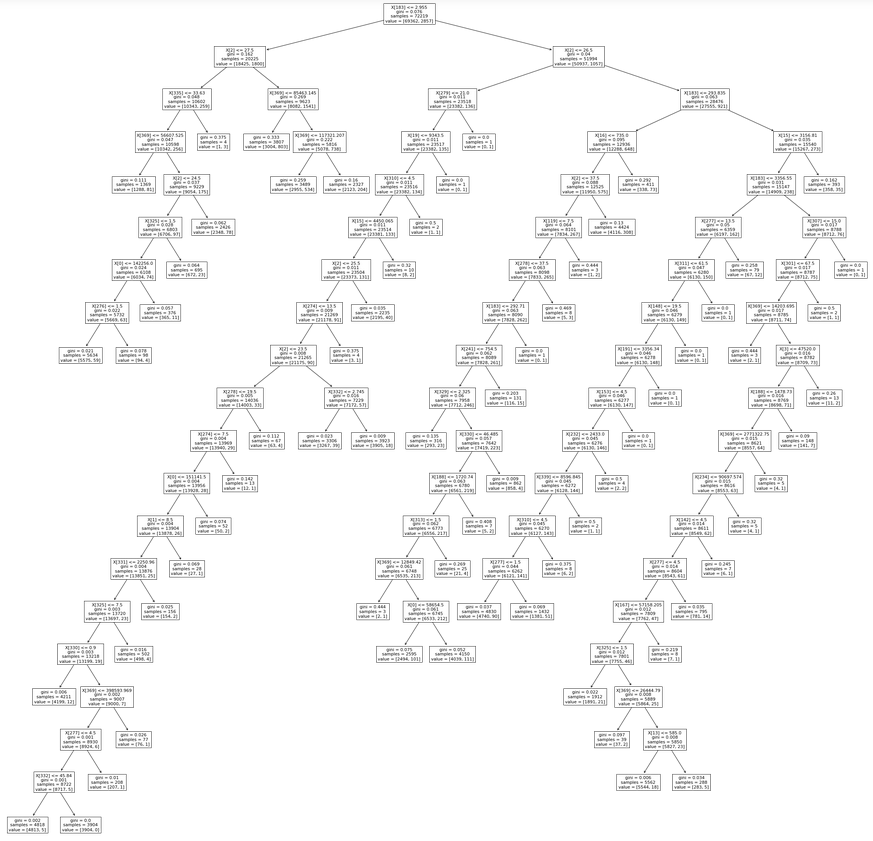
\includegraphics[width=6.5in]{model_3.png}
\end{figure}

Similar to Model 2, we continue to work with the \textit{min\_sample\_split} parameter. However, we have increased the value from 1,000 to 5,702. This number was chosen because it means that a leaf node cannot have more than 10\% of the original training sub-dataset. It allows for larger bins, which I originally hypothesized would create a more accurate, well-fit model. While the marginal returns of increasing the sample split quickly depreciated (this model also has a 96.0\% accuracy), it was worth testing to see the effect on GINI scores. I believed this model would have the best GINI scores not only for the training dataset, but for the test-dataset as well.

\subsection*{Model Four}
The fourth and final model uses the following parameters in the DecisionTreeClassifier function:

$$
DecisionTreeClassifier(min\_samples\_split=5702, max\_leaf\_nodes=15)
$$

A decision tree model using the parameters established in Model 4 can be visualized as so:

\begin{figure}[H]
	\centering
	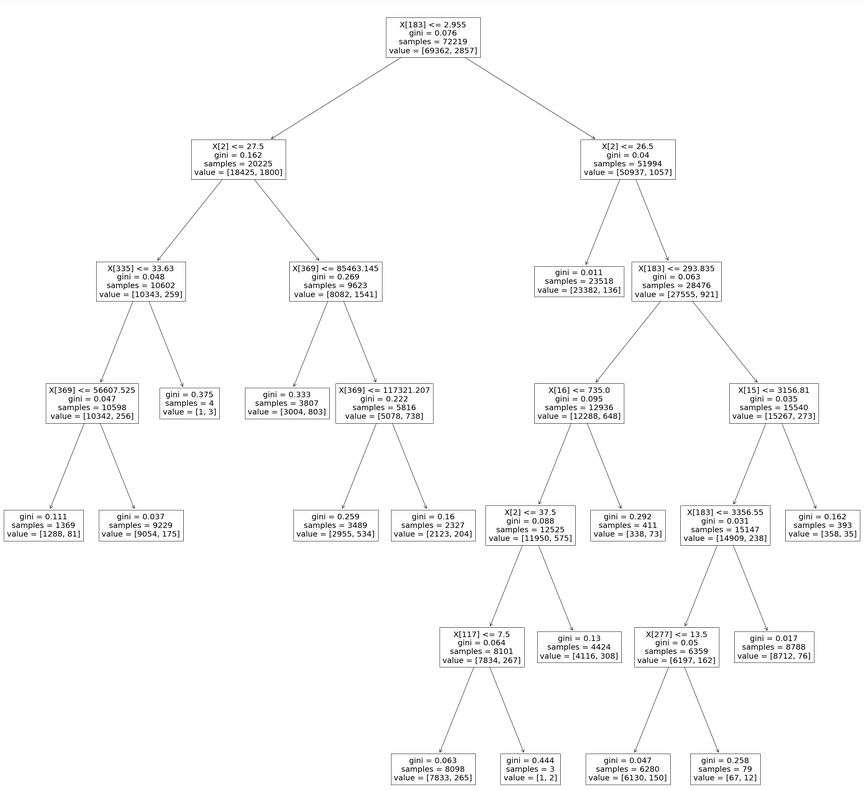
\includegraphics[width=6.5in]{model_4.png}
\end{figure}

This final model adds another parameter into our DecisionTreeClassifier function. Though the initial structure appears similar to Model 3, we now constrain the maximum number of leaf nodes to 15. This number was chosen admittedly relatively arbitrarily, but the goal is to choose a number smaller than the number of leaf nodes constructed in the previous model. The results from this model seemed to produce higher GINI scores but also return a slightly higher accuracy of 96.1\%. 

\section*{Conclusion}

\qquad \textbf{Model One Kaggle Score:} 0.55994

\qquad \textbf{Model Two Kaggle Score:} 0.50186

\qquad \textbf{Model Three Kaggle Score:} 0.49987

\qquad \textbf{Model Four Kaggle Score:} 0.49995

Interestingly enough, we reached the incredibly counter-intuitive conclusion that the best model was the one that had the fewest parameters established: Model 1. After spending time contemplating why that might be the case, the only logical conclusion would be that the parameters that I was establishing were working against the organic nature of the dataset. Theoretically, either Model 3 or 4 should have produced the most accurate results in the dataset, but it appears that the models I created were poor choices.

\section*{Improving the Models \& Kaggle Scores}
Potential ways to improve the model to get a higher score on Kaggle would be:

\qquad 1. Continue to change the parameters of the DecisionTreeClassifier function. The four models created here were models that tested different parameters of the DecisionTreeClassifier provided through sklearn. We could do parameter scanning, changing available features to see if we can see improvement. I believe this will only result in marginal improvements, and would consider finding alternative methods to improve the score.

\qquad 2. Hyperparameter tuning. Theoretically, hyperparameter tuning would be an effective way to tune even the DecisionTreeClassifier's parameters to see what would produce the optimal model. I would imagine that even creating a basic parameter grid using GridSearchCV (changing 'C' and 'gamma' values and assigning the verbose-ness of the search) could help us create a more accurate model.

\qquad 3. Using a different machine learning method. DecisionTreeClassifier and decision trees as a whole are a solid introduction to Machine Learning as a topic, but they may not necessarily be the most accurate model to use for this particular problem. Granted, this is the only model we've talked about in class and we were supposed to use it on this assignment, but I'm sure if we re-visited this exact same problem at the end of the year, we would produce better results using other methods.

\end{document}